% ------------------------------------------------------------------------------
% Chapter 4
% ------------------------------------------------------------------------------
\chapter{How to Improve Your Model Performance?}

\section{Improvement Strategies}
\label{sec:chap4 section 1}

After initial training, Model 3 showed promising results but still left room for improvement. To enhance the model's performance, several fine-tuning strategies were implemented. The ReduceLROnPlateau callback was used to monitor the validation accuracy, and the learning rate was reduced if the accuracy did not improve over ten epochs. This approach helped the model to converge more effectively by adjusting the learning rate dynamically. Additionally, ModelCheckpoint was utilized to save the best version of the model based on the minimum validation loss, ensuring that the most optimal weights were retained.

These fine-tuning efforts led to noticeable improvements in both training and validation accuracy and loss. As depicted in the accompanying plots, the training accuracy steadily increased, and the validation accuracy showed a more stable trend compared to the initial runs. The training loss decreased significantly, and although the validation loss exhibited some fluctuations, the overall trend was positive, indicating a better generalization capability of the model.

\section {Model Evaluation}
\label{sec:chap4 section 2}
With the best model we computed the confusion matrix and ROC curve. These are given in Figure ~\ref{fig:cha-4 figure1} and Figure ~\ref{fig:cha-4 figure2} respectively. The confusion matrix and ROC curve provide insights into the model's performance. The confusion matrix indicates that while the model correctly identifies a significant number of true positives (6154) and true negatives (12550), there is still a substantial number of false positives (3951) and false negatives (1492). This suggests that the model might benefit from further fine-tuning and potential adjustments in decision thresholds. The ROC curve, with an area under the curve (AUC) of 0.78, reflects a moderate level of discrimination between the positive and negative classes. While this is a promising start, aiming for a higher AUC by refining the model and its parameters will be crucial in improving overall accuracy and reliability.

\begin{figure}
    \centering
    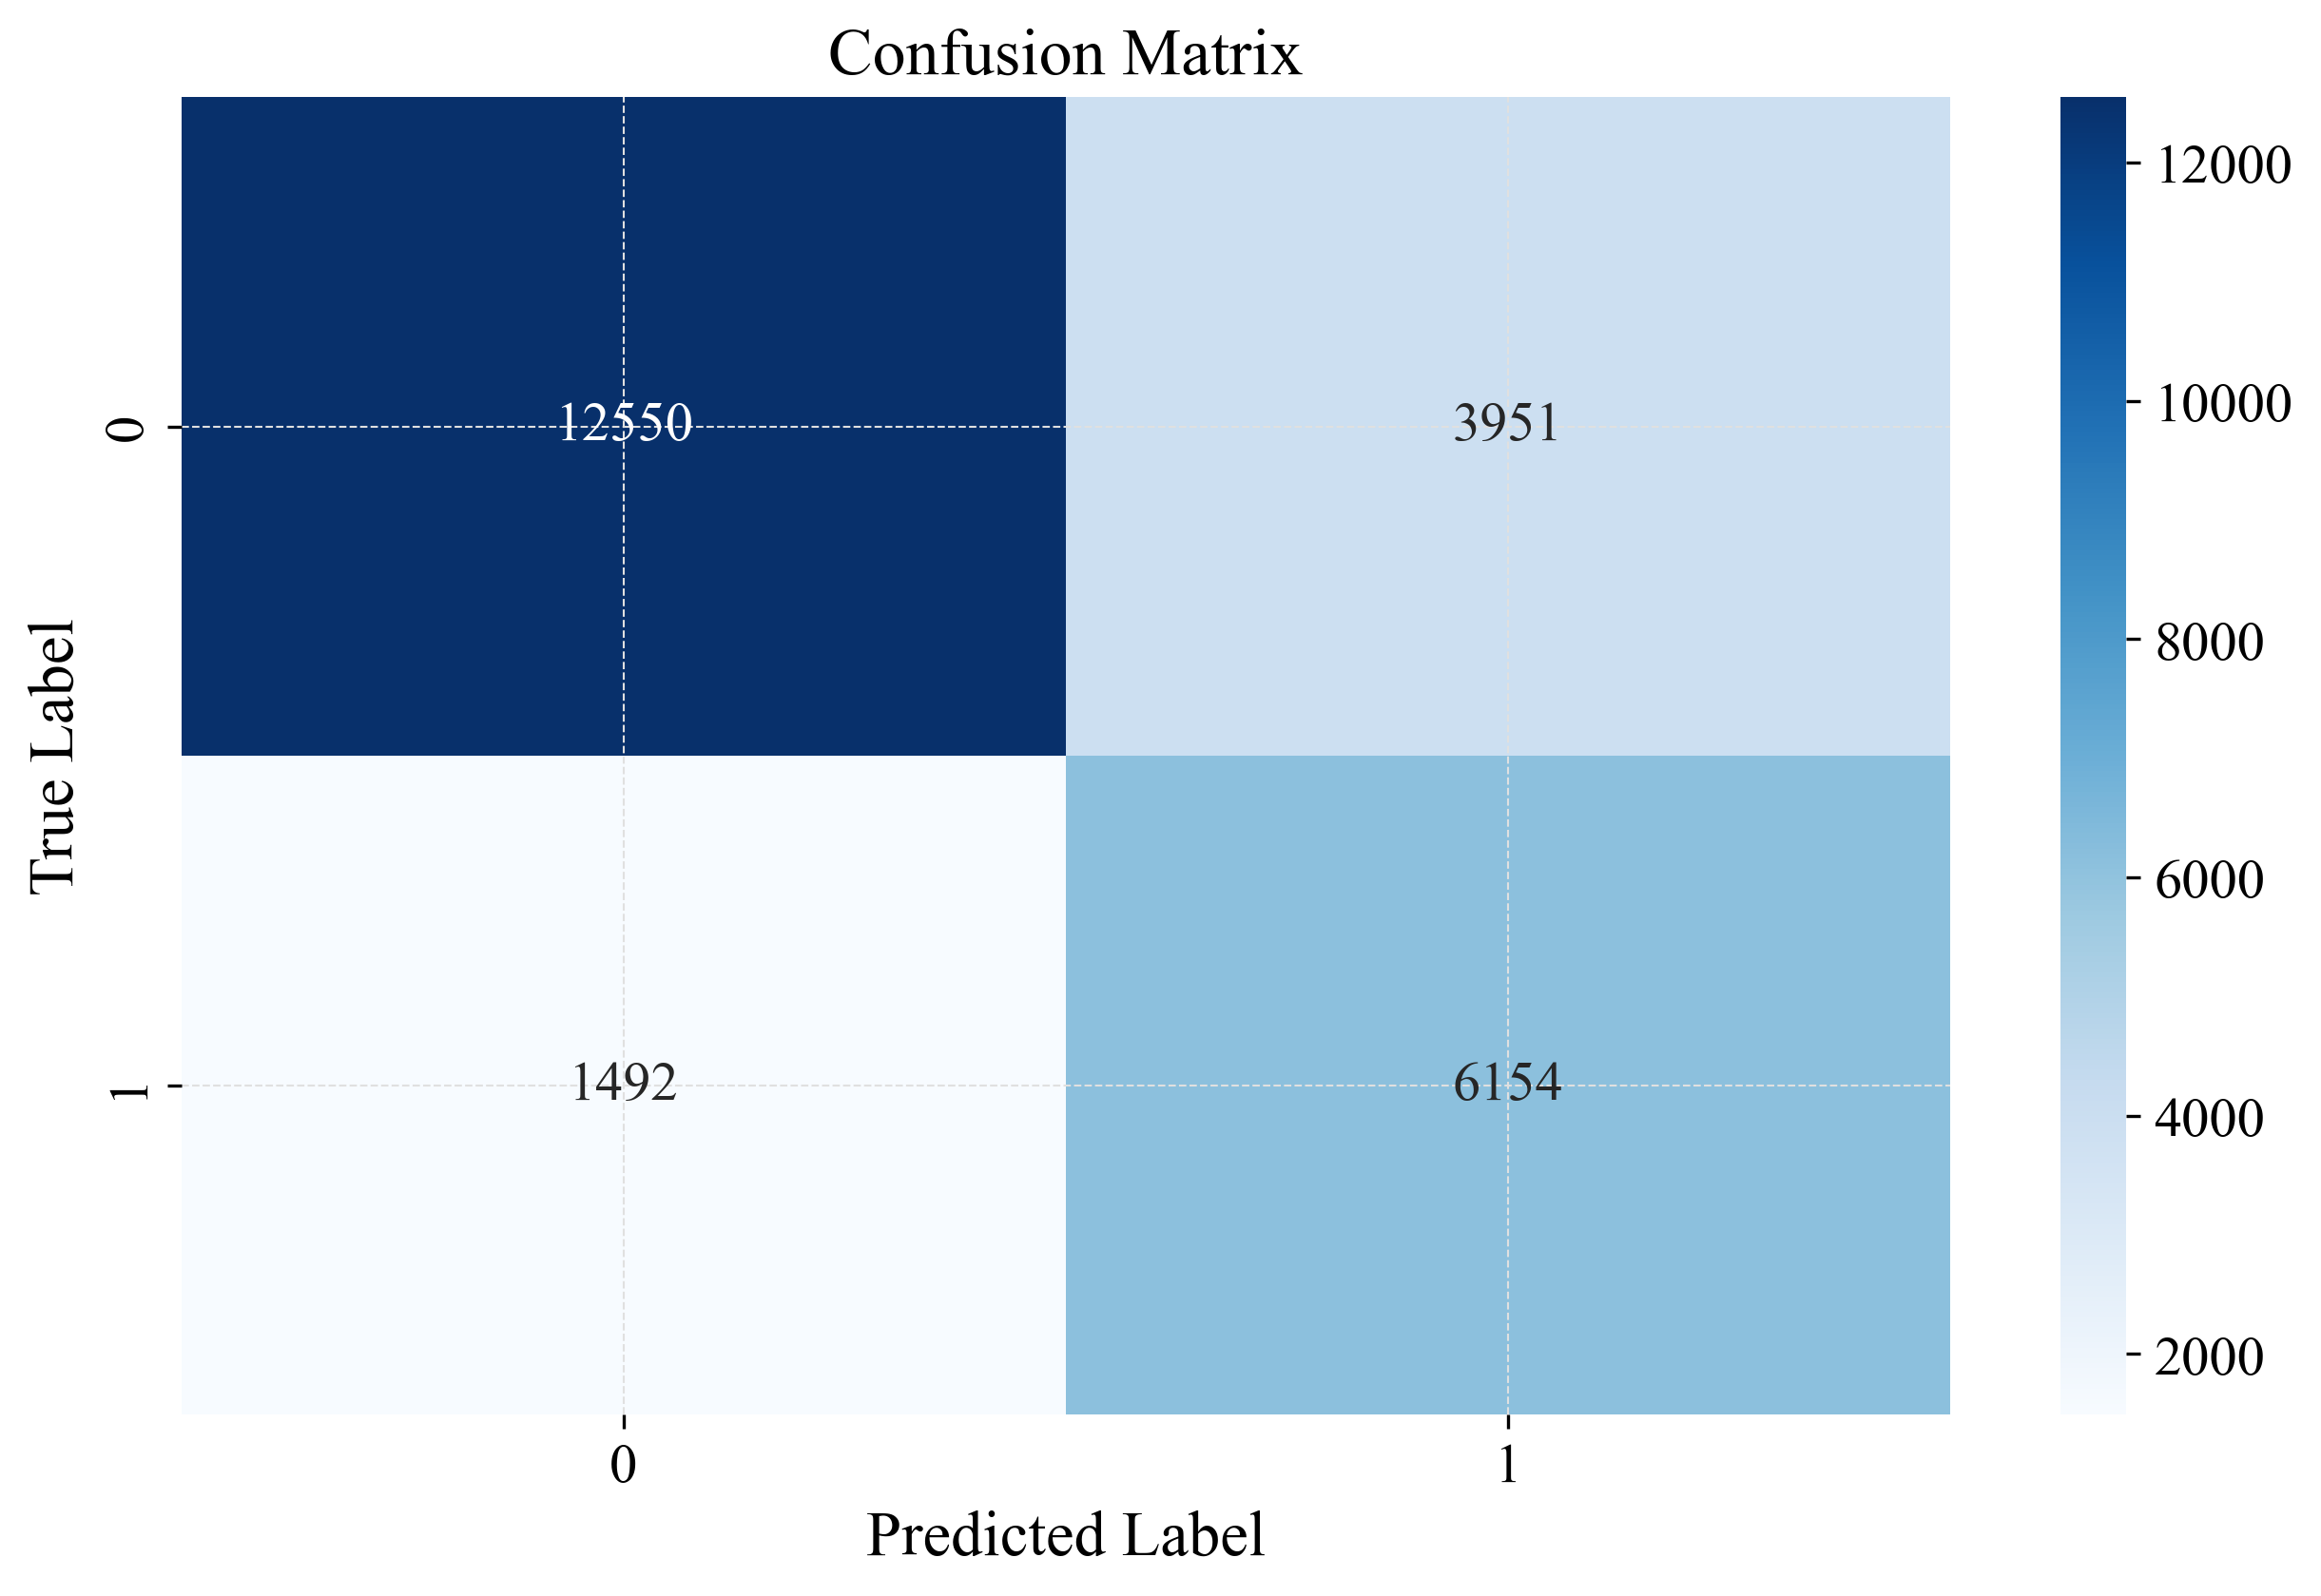
\includegraphics[width=0.8\textwidth]{figures/Figure33.png}
    \caption{Confusion Matrix for the Best Model}
    \label{fig:cha-4 figure1}
\end{figure}

\begin{figure}
    \centering
    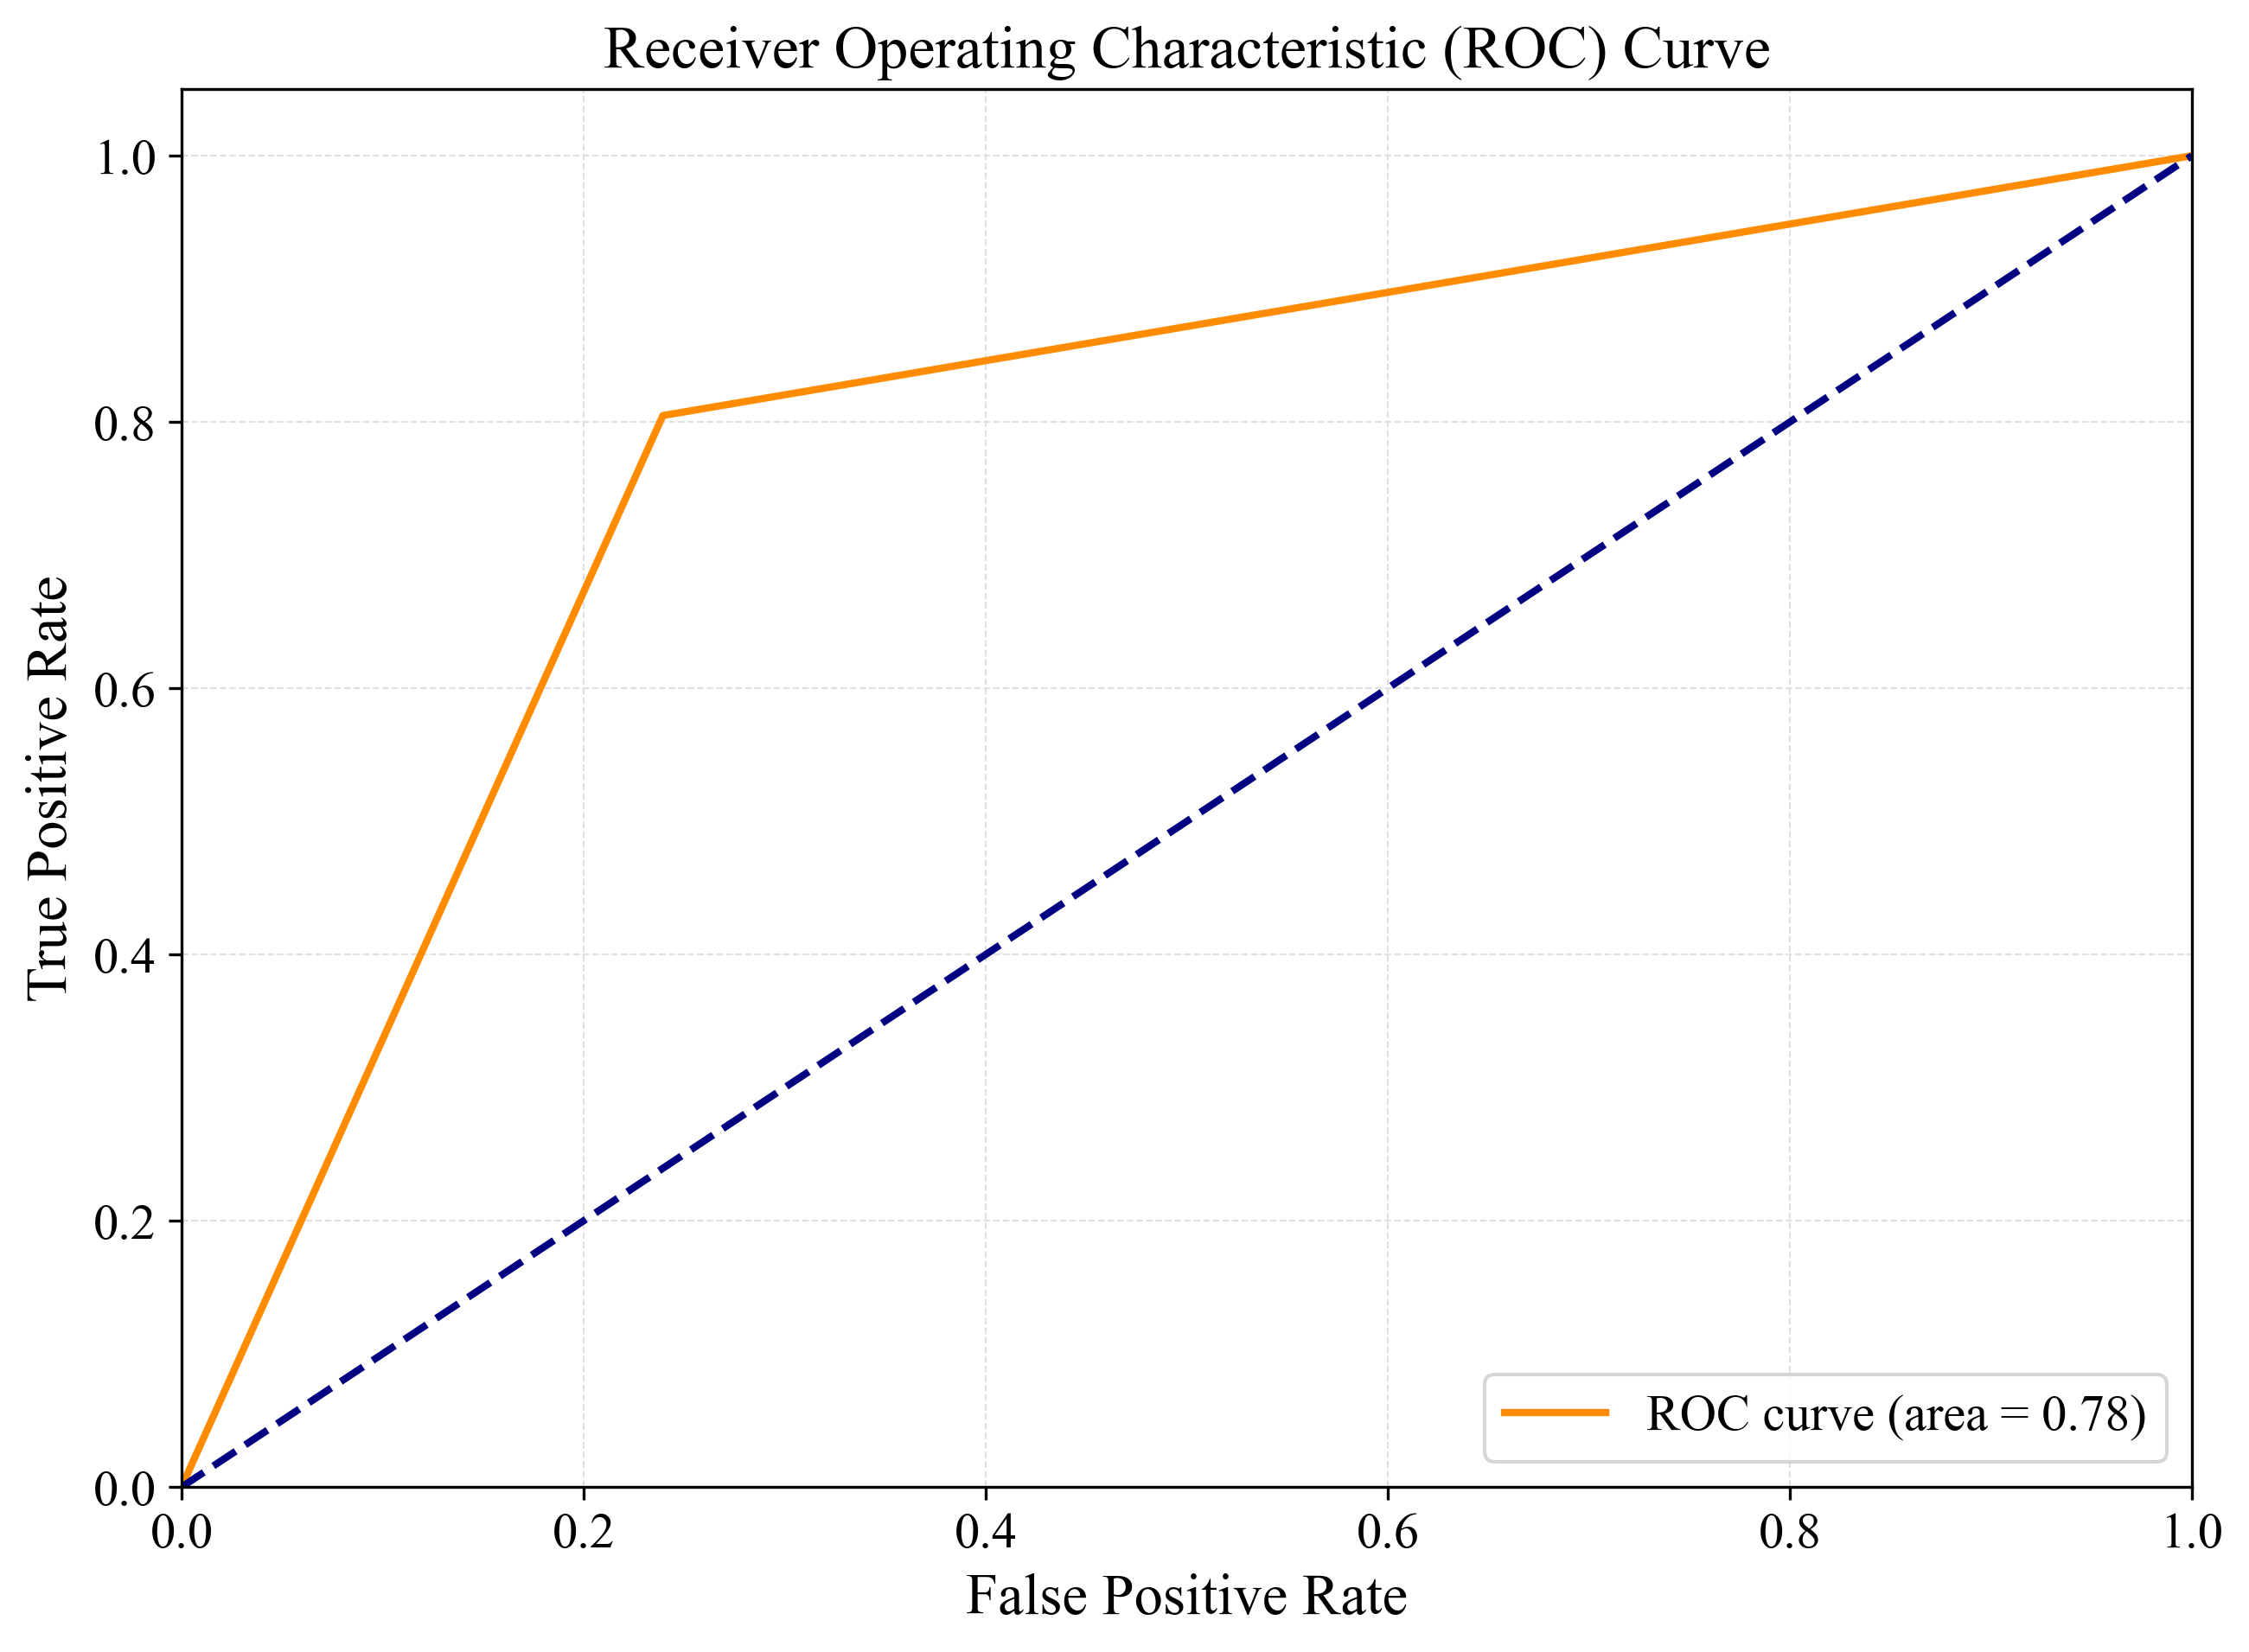
\includegraphics[width=0.8\textwidth]{figures/Figure34.png}
    \caption{ROC Curve for the Best Model}
    \label{fig:cha-4 figure2}
\end{figure}

\section{Future Steps}
\label{sec:chap4 section 3}

To further enhance the model's performance and prevent overfitting, several additional strategies can be considered (These are not implemented in the current model but can be explored in future iterations if time and resources permit):

\begin{itemize}
    \item \textbf{Data Augmentation:} Implementing advanced data augmentation techniques such as random rotations, translations, and horizontal flipping can help increase the diversity of the training data, making the model more robust.

    \item \textbf{Regularization:} Adding L2 regularization to the convolutional and dense layers can help prevent overfitting by penalizing large weights and encouraging simpler models.

    \item \textbf{Dropout Adjustment:} Experimenting with different dropout rates in the network can help determine the optimal level of regularization, ensuring that the model does not rely too heavily on any particular set of neurons.

    \item \textbf{Batch Normalization:} Integrating batch normalization layers can stabilize and accelerate the training process by normalizing the inputs to each layer, improving both training speed and model performance.

    \item \textbf{Learning Rate Scheduling:} Implementing advanced learning rate scheduling techniques such as cosine annealing or cyclic learning rates can help the model converge more efficiently and avoid local minima.

    \item \textbf{Ensemble Methods:} Training multiple models with different architectures and combining their predictions can lead to more robust and accurate results by leveraging the strengths of each individual model.

    \item \textbf{Transfer Learning:} Utilizing pre-trained models on similar datasets can provide a strong starting point, allowing the model to leverage learned features and improve performance with less training data.

    \item \textbf{Hyperparameter Tuning:} Conducting extensive hyperparameter tuning using techniques such as grid search or Bayesian optimization can help identify the optimal configuration for the model, leading to better performance.
\end{itemize}
